% debut d'un fichier latex standard
\documentclass[a4paper,12pt,twoside]{article}

\usepackage{lipsum}
\usepackage{empheq}

% pour l'inclusion de figures en eps,pdf,jpg
\usepackage{graphicx}
\usepackage{subcaption}
\usepackage{wrapfig}
% quelques symboles mathematiques en plus
\usepackage{amsmath}
\usepackage{amsthm} % Pour les preuves
\usepackage{cancel} % Pour barrer des trucs en mode math
% le tout en langue francaise
%\usepackage[french]{babel}
% on peut ecrire directement les caracteres avec l'accent
% a utiliser sur Linux/Windows
\usepackage[utf8]{inputenc}
\usepackage[T1]{fontenc}
% a utiliser sur le Mac
%\usepackage[applemac]{inputenc}
% pour l'inclusion de links dans le document
\usepackage[colorlinks,bookmarks=false,linkcolor=blue,urlcolor=blue]{hyperref}
\usepackage{siunitx}
% pour les degrés
\usepackage{textcomp}
\paperheight=297mm
\paperwidth=210mm

\setlength{\textheight}{235mm}
\setlength{\topmargin}{-1.2cm} % pour centrer la page verticalement
%\setlength{\footskip}{5mm}
\setlength{\textwidth}{15cm}
\setlength{\oddsidemargin}{0.56cm}
\setlength{\evensidemargin}{0.56cm}

\pagestyle{plain}

% quelques abreviations utiles
\def \be {\begin{equation}}
\def \ee {\end{equation}}
\def \dd  {{\rm d}}

\newcommand{\mail}[1]{{\href{mailto:#1}{#1}}}
\newcommand{\ftplink}[1]{{\href{ftp://#1}{#1}}}

\newcommand{\illabel}[1]{ ~ \refstepcounter{equation}(\theequation)\label{#1}} % Ecrit une équation dans le texte, numérotés.
\newcommand{\mbf}[1]{\mathbf{#1}} % bold font in math
\newcommand{\grad}[1]{\nabla#1}
\newcommand{\Div}[1]{\nabla\cdot\mathbf{#1}}
\newcommand{\rot}[1]{\nable\cross\mathbf{#1}}
\newcommand{\bracket}[1]{\left(#1\right)}
\newcommand{\sqbracket}[1]{\left[#1\right]}
\newcommand{\lapl}[1]{\Delta#1}

%
% latex SqueletteRapport.tex      % compile la source LaTeX
% xdvi SqueletteRapport.dvi &     % visualise le resultat
% dvips -t a4 -o SqueletteRapport.ps SqueletteRapport % produit un PostScript
% ps2pdf SqueletteRapport.ps      % convertit en pdf

% pdflatex SqueletteRapport.pdf    % compile et produit un pdf
% \message{================> TAILLE DE LA POLICE EN CM \printinunitsof{cm}\prntlen{\textwidth}}

% ======= Le document commence ici ======

\begin{document}
% Le titre, l'auteur et la date
\title{Quantum mechanics\\{\normalsize Harmonic oscillator, coupled harmonic oscillator, tunnel effect, uncertainty principle and detection of particles}\\{\small Physique Numérique I}\\{\small Rapport 8}}
\date{\today}
\author{Delphine Martres and Damien Korber\\{\small \mail{delphine.martres@epfl.ch} and \mail{damien.korber@epfl.ch}}}

\maketitle
\tableofcontents % Table des matieres


% Quelques options pour les espacements entre lignes, l'identation
% des nouveaux paragraphes, et l'espacement entre paragraphes
\baselineskip=16pt
\parindent=15pt
\parskip=5pt
\newpage

%%%% ON COMMENCE A ECRIRE D'ICI

%===============================================================================
%=============================== INTRODUCTION ==================================
%===============================================================================
\section{Introduction}
%TODO : Mettre l'équation de Schrödinger (\label{eq:schrödinger_eq}) et sa solution (\label{eq:schrödinger_sol}).

\section{Implementation}\label{sec:impl}
  This first section will focus on the numerical implementation of the problem.

  \subsection{Semi-implicit Crank-Nicholson's numerical method}
    First, the time needs to be discretized: $t_j = t_0 + j\Delta t$.
    Now, apply this discretization to the solution of Schrödinger's equation (Eq. \eqref{eq:schrödinger_sol}), which leads to equation \eqref{eq:schrödinger_sol_disc}.

    \begin{equation}
      \psi(\mbf{x}, t + \Delta t) = \exp\bracket{-\frac{i}{\hbar}\Delta t H}\psi(\mbf{x}, t)
      \label{eq:schrödinger_sol_disc}
    \end{equation}

    By multiplying both sides by $\exp\bracket{\frac{i}{\hbar}\frac{\Delta t}{2}H}$, and by using a limited development, equation \eqref{eq:crank-nicholson} follows, which is Crank-Nicholson's semi-implicit numerical method.

    \begin{equation}
      \bracket{1 + \frac{i}{\hbar}\frac{\Delta t}{2}H}\psi(\mbf{x}, t + \Delta t) = \bracket{1 - \frac{i}{\hbar}\frac{\Delta t}{2}H}\psi(\mbf{x}, t)
      \label{eq:crank_nicholson}
    \end{equation}



  \subsection{Construction of matrices H, A and B and implementation of the border conditions}
    \subsubsection{Construction of H}\label{sec:constr_H}
      The hamiltonian $H(\psi)$ is given by equation \eqref{eq:hamiltonian_cont}.

      \begin{equation}
        H(\psi) = -\frac{\hbar^2}{2m}\nabla^2\psi + V(\mbf{x})\psi
        \label{eq:hamiltonian_cont}
      \end{equation}

      By discretizing the space using a finite difference method (Eq. \eqref{eq:disc_space}), the hamiltonian can be rewritten as a tridiagonal matrix given by \eqref{eq:hamiltonian_matrix}, where $d_i$ is the diagonal, $a_i$ is the subdiagonal and $c_i$ is the superdiagonal.

      \begin{equation}
        \bracket{\frac{\partial^2\psi}{\partial x^2}}_j = \frac{\psi_{j-1} - 2\psi_j + \psi_{j+1}}{\bracket{\Delta x}^2}
        \label{eq:disc_space}
      \end{equation}

      \begin{equation}
        H: \begin{cases}
          a_i &= -\frac{\hbar^2}{2m(\Delta x)^2}\\
          d_i &= \frac{\hbar^2}{m(\Delta x)^2} + V(x)\\
          c_i &= -\frac{\hbar^2}{2m(\Delta x)^2}\\
        \end{cases}
        \label{eq:hamiltonian_matrix}
      \end{equation}

    \subsubsection{Construction of A and B}
      In Crank-Nicholson's semi-implicit method (Eq. \eqref{eq:crank_nicholson}), and by using the matrix H, matrices A and B can be identified as the left hand side respectively the right hand side.
      Matrices A and B are both tridiagonal matrices, where $d_i^A$ and $d_i^B$ are the diagonals, $a_i^A$ and $a_i^B$ are the subdiagonals and $c_i^A$ and $c_i^B$ are the overdiagonals.
      To summary, A and B are identified as given by equation \eqref{eq:A_B_identification}.

      \begin{equation}
        \begin{cases}
          A = I + \frac{i}{\hbar}\frac{\Delta t}{2}H \\
          B = I - \frac{i}{\hbar}\frac{\Delta t}{2}H
        \end{cases}
        \label{eq:A_B_identification}
      \end{equation}

      where $I$ is the identity matrix.
      All the terms of A and B are expressed as given by equation \eqref{eq:terms_A_B}.

      \begin{equation}
        \begin{cases}
          a_i^A &= \frac{i\Delta t}{2\hbar} a_i\\
          a_i^B &= -\frac{i\Delta t}{2\hbar} a_i\\
          d_i^A &= 1 + \frac{i\Delta t}{2\hbar} d_i\\
          d_i^B &= 1 - \frac{i\Delta t}{2\hbar} d_i\\
          c_i^A &= \frac{i\Delta t}{2\hbar} c_i\\
          c_i^B &= -\frac{i\Delta t}{2\hbar} c_i\\
        \end{cases}
        \label{eq:terms_A_B}
      \end{equation}

      with $d_i$, $a_i$ and $c_i$ defined by equation \eqref{eq:hamiltonian_matrix}.
      By defining the vector ($\mbf{\psi}^k(\mbf{x}))_i = \mbf{\psi}_i^k = \psi(x_i, t_k)$, equation \eqref{eq:crank_nicholson_matrix} follows.

      \begin{equation}
        A\mbf{\psi}^{k+1}(\mbf{x}) = B\mbf{\psi}^k(\mbf{x})
        \label{eq:crank_nicholson_matrix}
      \end{equation}


    \subsubsection{Border conditions}
      The border condition is given by $\psi(x_1 = x_L, t_k) = \psi(x_N = x_R, t_k) = 0$.
      The implementation used does not allow a modification of $\psi$, which implies that the conditions must be applied to matrices A and B.
      By computing the first and last equation obtain from equation \eqref{eq:crank_nicholson_matrix} at $t=t_k$, equation \eqref{eq:border_cond_eq} follows.

      \begin{equation}
        \begin{cases}
          d_1^A\psi_1^{k+1} +c_1^A\psi_2^{k+1} = \overbrace{d_1^B\psi_1^k}^\text{=0 from border condition} + c_1^B\psi_2^k\\
          a_{N-1}^A\psi_{N-1}^{k+1} + d_N^A\psi_N^{k+1} = a_{N-1}^B\psi_{N-1}^k + \underbrace{d_N^B\psi_N^k}_\text{=0 from border condition}
        \end{cases}
        \label{eq:border_cond_eq}
      \end{equation}

      Thus, to obtain $\psi_1^{k+1} = \psi_N^{k+1} = 0$, simply set $c_1^A = c_1^B = a_{N-1}^A = a_{N-1}^B = 0$ and $d_1^A = d_N^A = 1$, which leads to the border conditions.

  \subsection{Initial wave function}
    The equation for the initial wave function is given by:
    \begin{equation}
     \psi(x,0)=\exp(ik_0x)\exp\left[-(x-x_0)^2/(2\sigma_0^2)\right]
     \label{eq:psiinit}
    \end{equation}
    with $k_0=2\pi n/(x_R-x_L)$, $\sigma_0=\sigma_{norm}(x_R-x_L)$. $x_0$, $n$ and $\sigma_{norm}$ are given. In the algorithm, it is simply written as:
    \begin{equation}
     \psi_j=\exp(ik_0x_j)\exp\left[-(x_j-x_0)^2/(2\sigma_0^2)\right]
     \label{eq:psiinitdis}
    \end{equation}

  \subsection{Probability function}
    The probability that the particle is situated between points $n_L\Delta x$ and $n_R\Delta x$ is given by the following integral:
    \begin{equation}
     P_{nL,nR} = \int_{n_L\Delta x}^{n_R\Delta x} |\psi(x,t)|^2 dx
    \end{equation}

    To compute this probability and all following integrals with respect to $x$, the trapezoidal rule will be used.\\
    An estimation of the integral of any integrable function $g$ can be found using the trapezoidal rule, which is given by equation \eqref{eq:trapeze-rule}.

    \begin{equation}
      \int_a^b g(x)dx \approx h\sum_{i=1}^N\bracket{\frac{g(x_i) + g(x_{i+1})}{2}}
      \label{eq:trapeze-rule}
    \end{equation}
    with $h = \Delta x$.

    In this case, we get:
    \begin{equation}
     P_{nL,nR}=\frac{\Delta x}{2}\sum_{i=n_L}^{n_R-1} |\psi_i|^2+|\psi_{i+1}|^2
    \end{equation}


  \subsection{Energy}
    The computation of the energy of a particle is given by the mean of the Hamiltonian, which is given by equation \eqref{eq:energy_def}.

    \begin{equation}
      E(t) = \langle H \rangle(t) = \int_{x_L}^{x_R}\psi^*(x,t)H(x)\psi(x,t)dx
      \label{eq:energy_def}
    \end{equation}

    By using the results from equation \eqref{eq:hamiltonian_matrix}, the vector definition of $\psi$ and the trapezoidal rule (eq. \eqref{eq:trapeze-rule}), the energy can be computed.

    First, we need to compute $H\psi$, which is given by equation \eqref{eq:H*psi}.

    \begin{align}
      \begin{split}
        (H\mbf{\psi})_i &= a_{i-1}\psi_{i-1} + d_i\psi_i + c_i\psi_{i+1} \text{ for } i\in[2, N-1]\\
        (H\mbf{\psi})_1 &= d_1\psi_1 + c_1\psi_2 \\
        (H\mbf{\psi})_N &= a_{N-1}\psi_{N-1} + d_N\psi_N
      \end{split}
      \label{eq:H*psi}
    \end{align}

    Then, the energy is given by equation \eqref{eq:energy}.

    \begin{equation}
      E(t) = \frac{\Delta x}{2}\sum_{i=1}^{N-1} (\mbf{\psi}_i^k)^*(H\mbf{\psi})_i + (\mbf{\psi}_{i+1}^k)^*(H\mbf{\psi})_{i+1}
      \label{eq:energy}
    \end{equation}

  \subsection{Average position}
  The average position of the particle is given by:
  \begin{equation}
   \langle x \rangle(t) = \int_{x_L}^{x_R}\psi^*(x,t)x\psi(x,t)dx
  \end{equation}
  and in its dicretized form:
  \begin{equation}
   \langle x \rangle(t) = \frac{\Delta x}{2} \sum_{i=1}^{N} \psi_i^*x_i\psi_i + \psi_{i+1}^*x_{i+1}\psi_{i+1}
  \end{equation}\\
  The average $x^2$ of the particle is given by:
  \begin{equation}
   \langle x^2 \rangle(t) = \int_{x_L}^{x_R}\psi^*(x,t)x^2\psi(x,t)dx
  \end{equation}
  and in its dicretized form:
  \begin{equation}
   \langle x^2 \rangle(t) = \frac{\Delta x}{2} \sum_{i=1}^{N} \psi_i^*x_i^2\psi_i + \psi_{i+1}^*x_{i+1}^2\psi_{i+1}
  \end{equation}
  
  \subsection{Average momentum}
  The average momentum of the particle is given by:
  \begin{equation}
   \langle p \rangle(t) = \int_{x_L}^{x_R}\psi^*(x,t)\left(-i\hbar\frac{\partial\psi(x,t)}{\partial x}\right)dx
  \end{equation}
  and by using the finite central differences for the derivative
  \begin{equation*}
   \left(\frac{\partial\psi}{\partial x}\right)_i = \frac{\psi_{i+1}-\psi_{i-1}}{2\Delta x}
  \end{equation*}%TODO: clarifier la consigne sur les pts de maillage aux extrémités.
  
  \subsection{Uncertainty calculation}
  The uncertainties on the position and the momentum are respectively given by:
  \begin{align}
   &\langle \Delta x\rangle(t) = \sqrt{\langle x^2 \rangle - \langle x \rangle^2}\\
   &\langle \Delta p\rangle(t) = \sqrt{\langle p^2 \rangle - \langle p \rangle^2}
  \end{align}


\section{Algorithm test with an harmonic oscillator}\label{sec:har_osc} %TODO : Dans TOUTE cette section, il faut changer la légende des graphes. Elles sont plus ou moins toutes fausses. Genre y'a les unités et tout le bordel qui match pas.
  In this section, the implementation detailed on section \ref{sec:impl} will be tested on a simple harmonic oscillator.
  The parameters are $x_L=\num{-200}$, $x_R=\num{200}$, $\omega = \num{0.003}$, $\Delta = 0$, $x_0 = 0$, $\sigma_\text{norm} = 0.06$, $n=14$ and $t_\text{fin} = 5000$. %TODO : C'est quoi les unités dans ce projet ? Y'a rien qu'est décrit et j'ai l'impression que c'est pas clair.

  \subsection{Convergence studies}
    By taking $N_\text{inters} = 300$, multiple convergence studies will be done.\\

    The results are given by figure \ref{fig:i_conv}.

    \begin{figure}[h]
      \centering
      \begin{subfigure}{0.45\textwidth}
        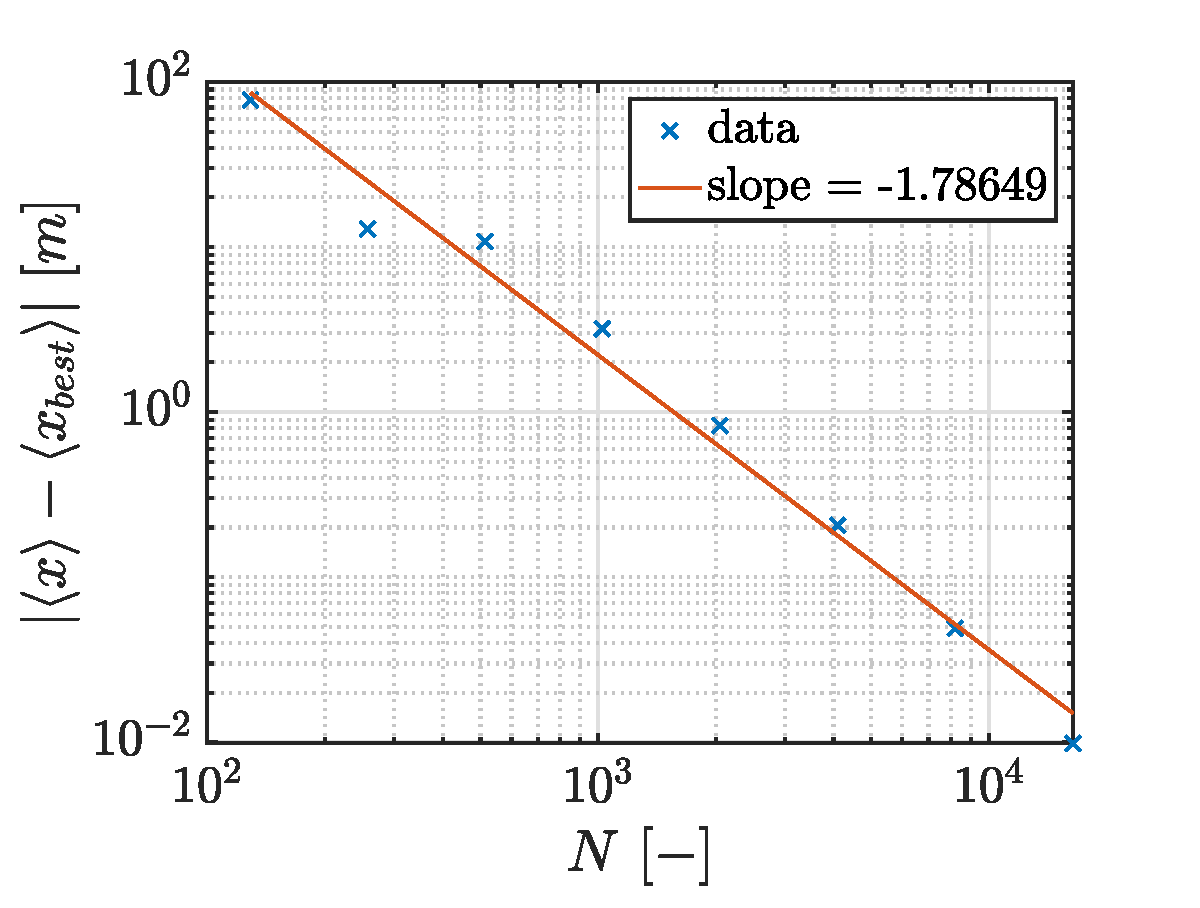
\includegraphics[width=\textwidth]{graphs/i_conv_x.eps}
        \caption{$\langle x \rangle (t)$}
        \label{fig:i_conv_x}
      \end{subfigure}
      ~
      \begin{subfigure}{0.45\textwidth}
        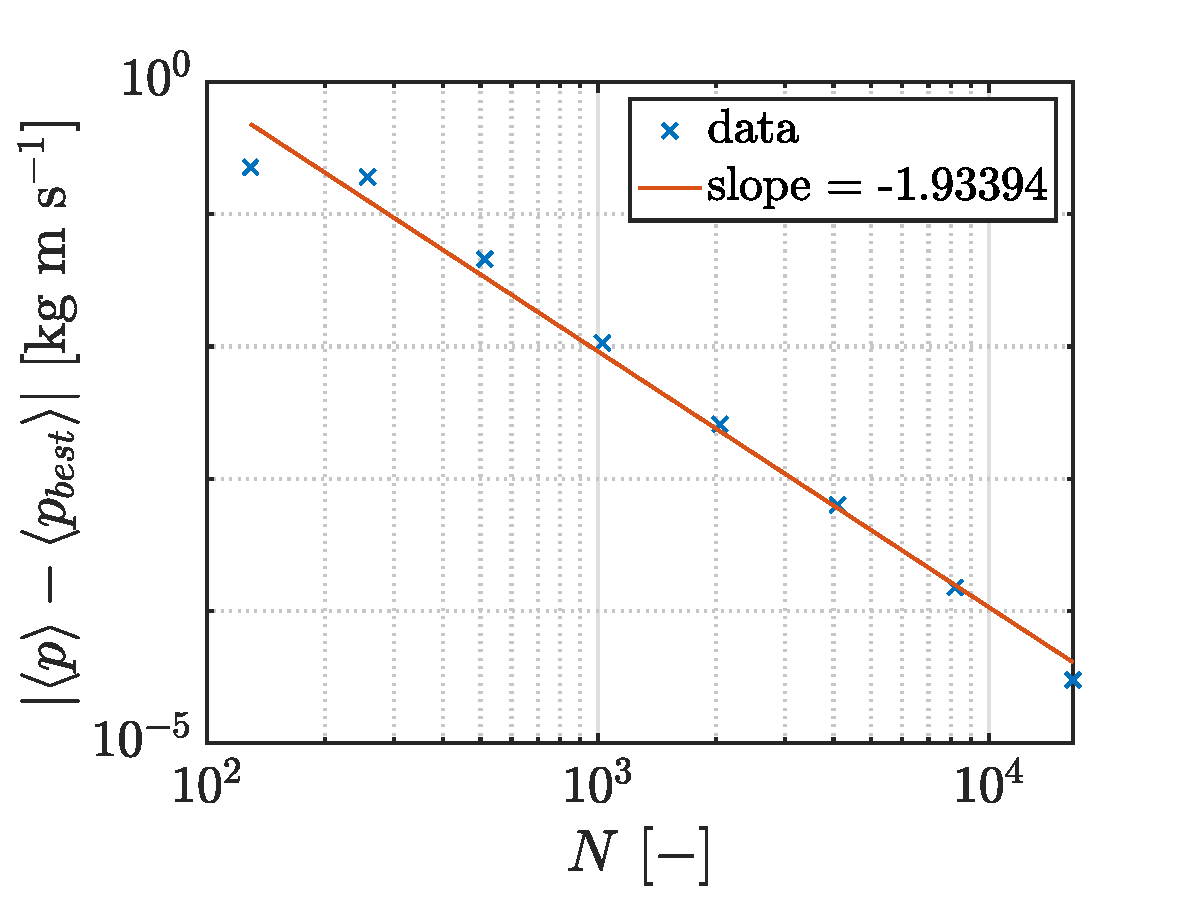
\includegraphics[width=\textwidth]{graphs/i_conv_p.eps}
        \caption{$\langle p \rangle (t)$}
        \label{fig:i_conv_p}
      \end{subfigure}
      ~
      \begin{subfigure}{0.45\textwidth}
        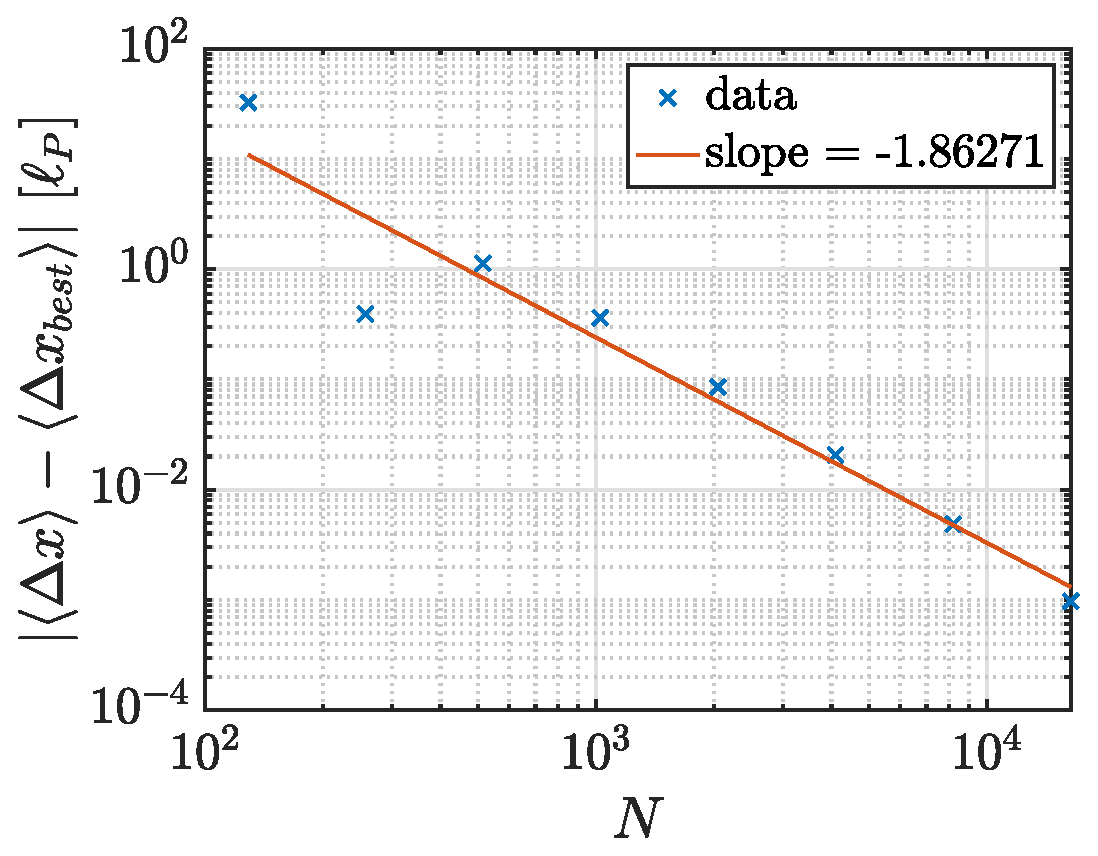
\includegraphics[width=\textwidth]{graphs/i_conv_dx.eps}
        \caption{$\langle \Delta x \rangle (t)$}
        \label{fig:i_conv_dx}
      \end{subfigure}
      ~
      \begin{subfigure}{0.45\textwidth}
        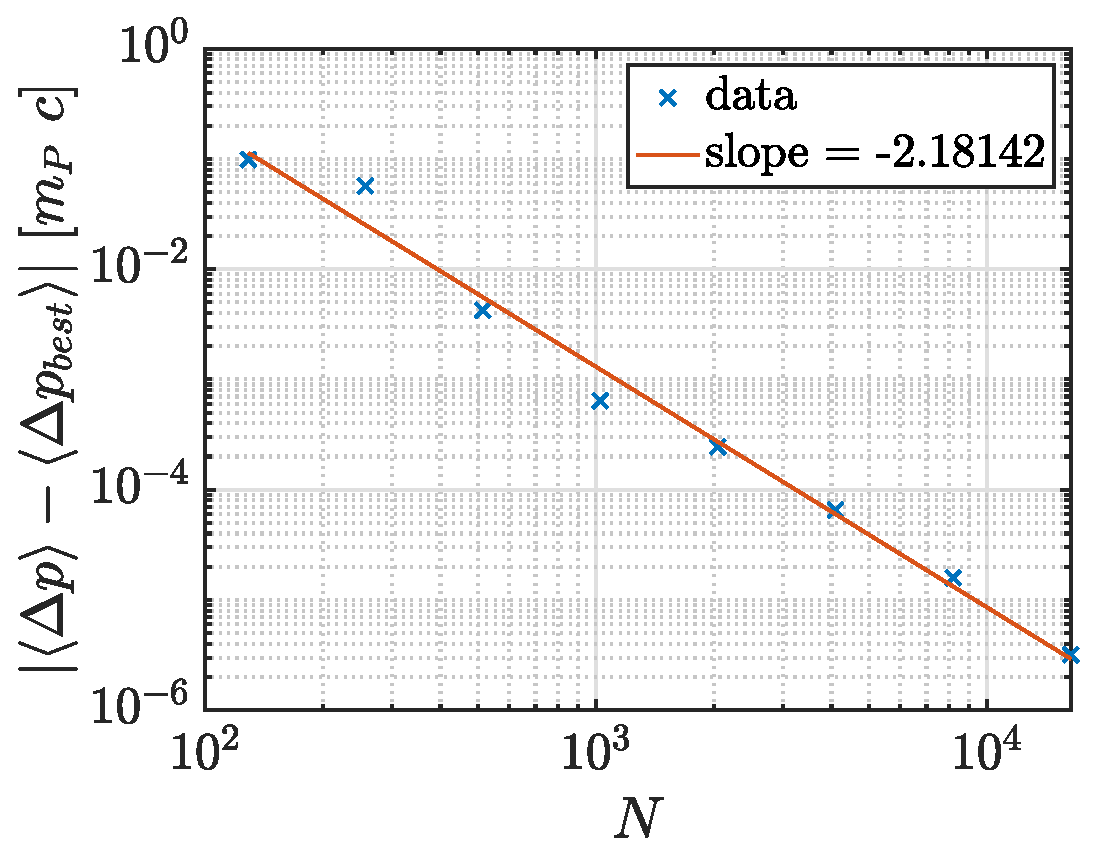
\includegraphics[width=\textwidth]{graphs/i_conv_dp.eps}
        \caption{$\langle \Delta p \rangle (t)$}
        \label{fig:i_conv_dp}
      \end{subfigure}
      \caption{Convergence study on multiple quantities with respect to $\Delta t$, with $N\in[\num{129}, \num{16380}]$ and $\Delta t = \num{5000}/N$. All the values are taken at t=5000.}
      \label{fig:i_conv}
    \end{figure}

    Figure \ref{fig:i_conv} gives the convergence study on the mean position $\langle x \rangle$ (Fig. \ref{fig:i_conv_x}), the mean momentum $\langle p \rangle$ (Fig. \ref{fig:i_conv_p}), the mean position uncertainty $\langle \Delta x \rangle$ (Fig. \ref{fig:i_conv_dx}) and the mean momentum uncertainty $\langle \Delta p \rangle$ (Fig. \ref{fig:i_conv_dp}).
    These resuts show that the numerical method approximately converges on the 2nd order.
    %TODO : Je sais pas quoi dire. :|


  \subsection{Total probability}
    The second verification is that the total probability verifies $\Sigma_i P_i(t) = 1~\forall t$.\\

    Figure \ref{fig:i_ptot} indeed shows that the sum of the left side probability and the right side probability equals 1.
    This figures also shows how the probability of both sides evolve over time, and it can be seen that the position oscillates on both sides.

    \begin{figure}[h]
      \centering
      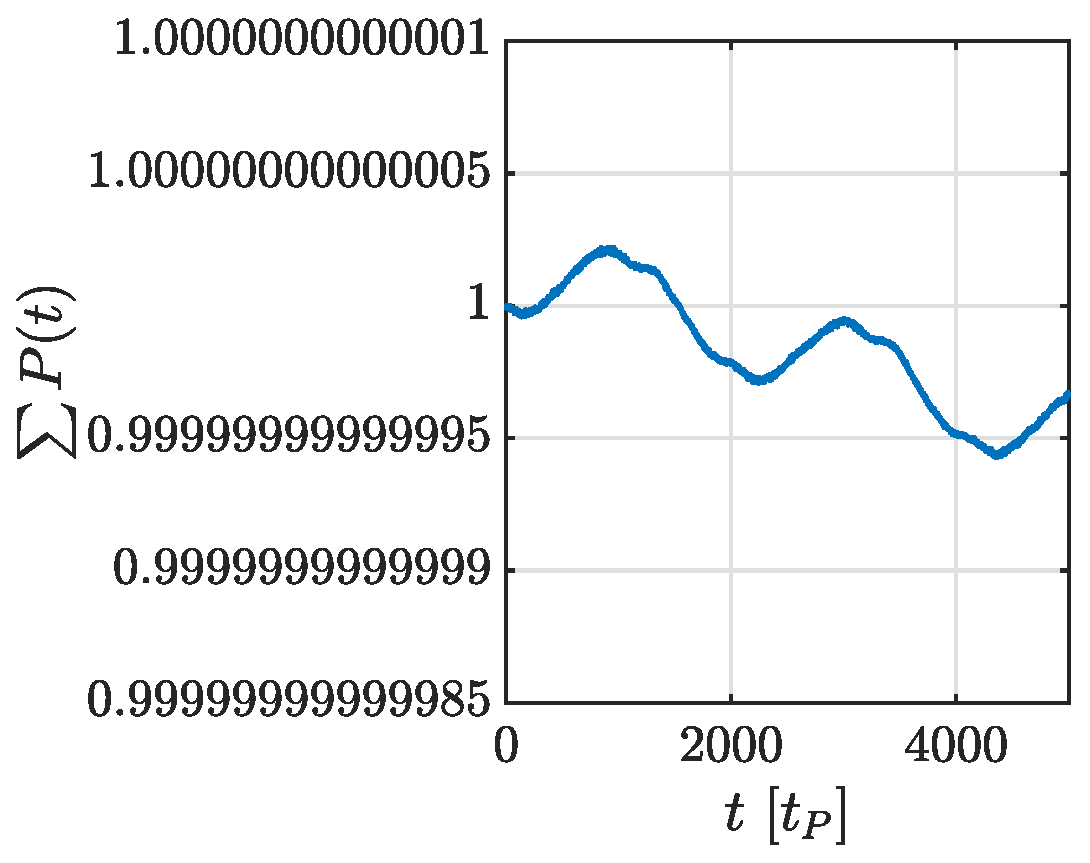
\includegraphics[width=0.5\textwidth]{graphs/i_ptot.eps}
      \caption{sum of probabilities over time, $\Delta t = 1$}
      \label{fig:i_ptot}
    \end{figure}


  \subsection{Conservation of mean energy}
    The third verification is that the mean energy is conserved over time.\\

    Figure \ref{fig:i_E} shows that the mean energy is more or less conserved.
    However, it can be observed that it slightly reduces over time, but this is neglectable, as the difference is too small to be shown on the y-axis. This is probably the result of numerical roundings, which always appears when using numerical methods.

    \begin{figure}[h]
      \centering
      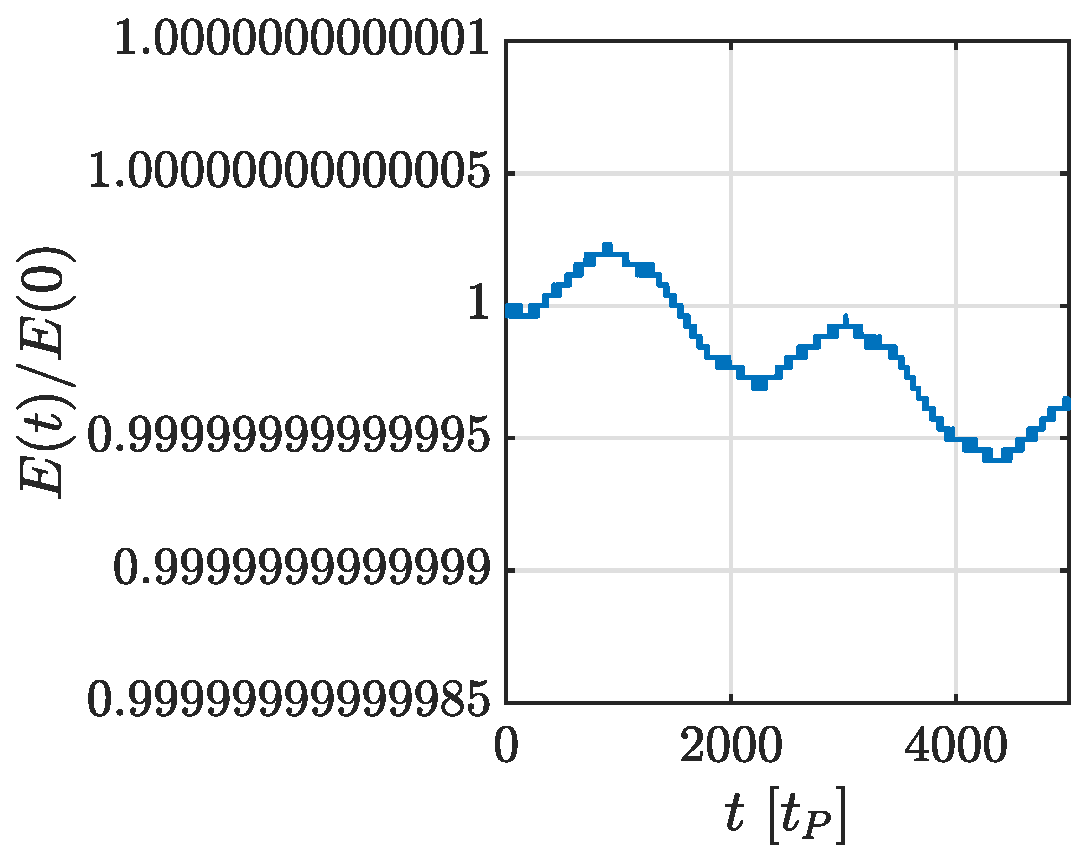
\includegraphics[width=0.8\textwidth]{graphs/i_E.eps}
      \caption{mean energy over time, $\Delta t = 1$}
      \label{fig:i_E}
    \end{figure}

  \subsection{Heisenberg's uncertainty principle}
    This last part focuses on the verification of the correctness of Heisenberg's uncertainty principle which states that $\forall t:~\langle \Delta x \rangle(t)\cdot\langle \Delta p \rangle(t) \geq \frac{\hbar}{2}$. Note that, as stated before, a normalized $\hbar$ has been taken, which gives $\hbar=1$.\\

    The result is given by figure \ref{fig:i_heisenberg} and shows that the principle is overall verified.
    %TODO : Parler du fait que le théorème est plus ou moins vérifié, mais que y'a quand même des parties qui posent problème.

    \begin{figure}[h]
      \centering
      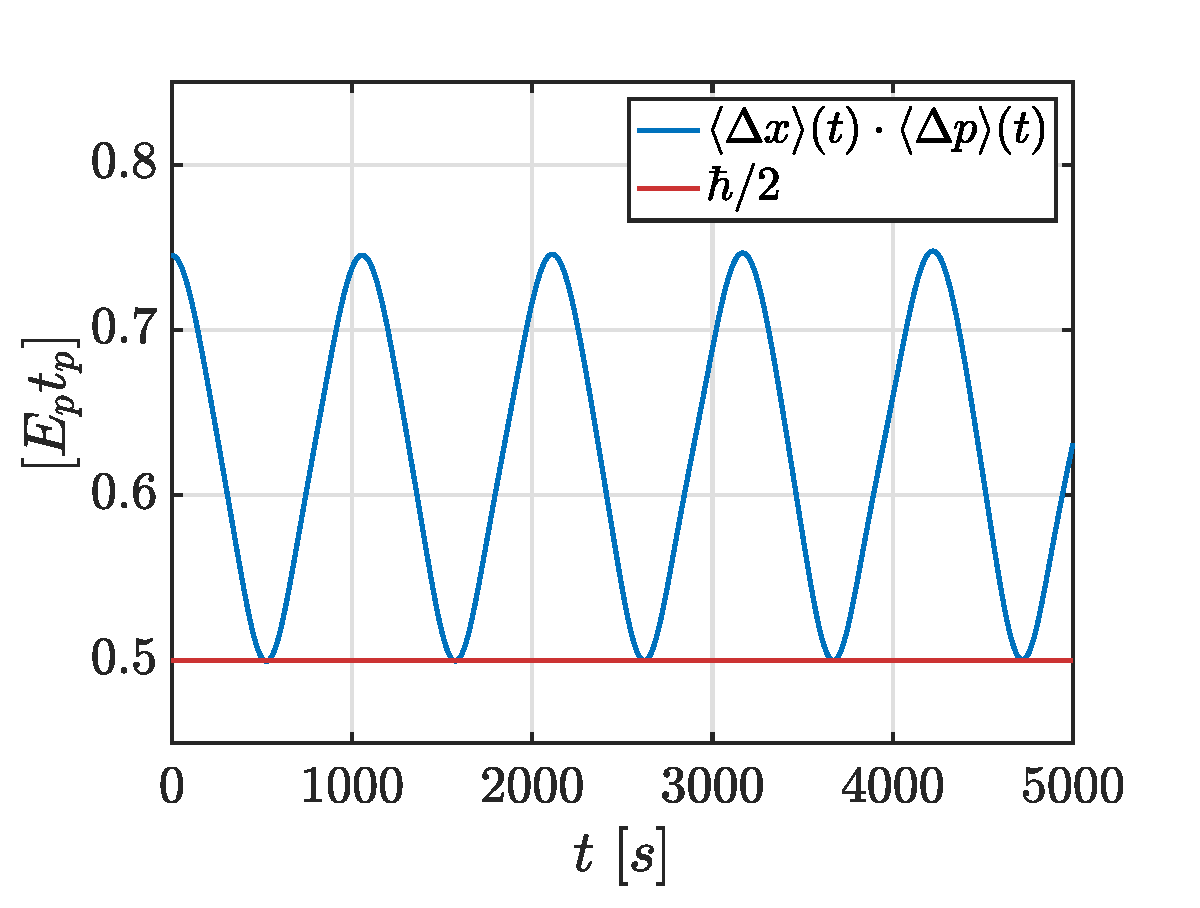
\includegraphics[width=0.5\textwidth]{graphs/i_heisenberg.eps}
      \caption{CAPTION A METTRE TUT}
      \label{fig:i_heisenberg}
    \end{figure}




\section{Mean movement analysis for a particle and comparison with the classic case}


\section{Tunnel effect}

\begin{figure}[h]
  \centering
  \begin{subfigure}[t]{0.45\textwidth}
    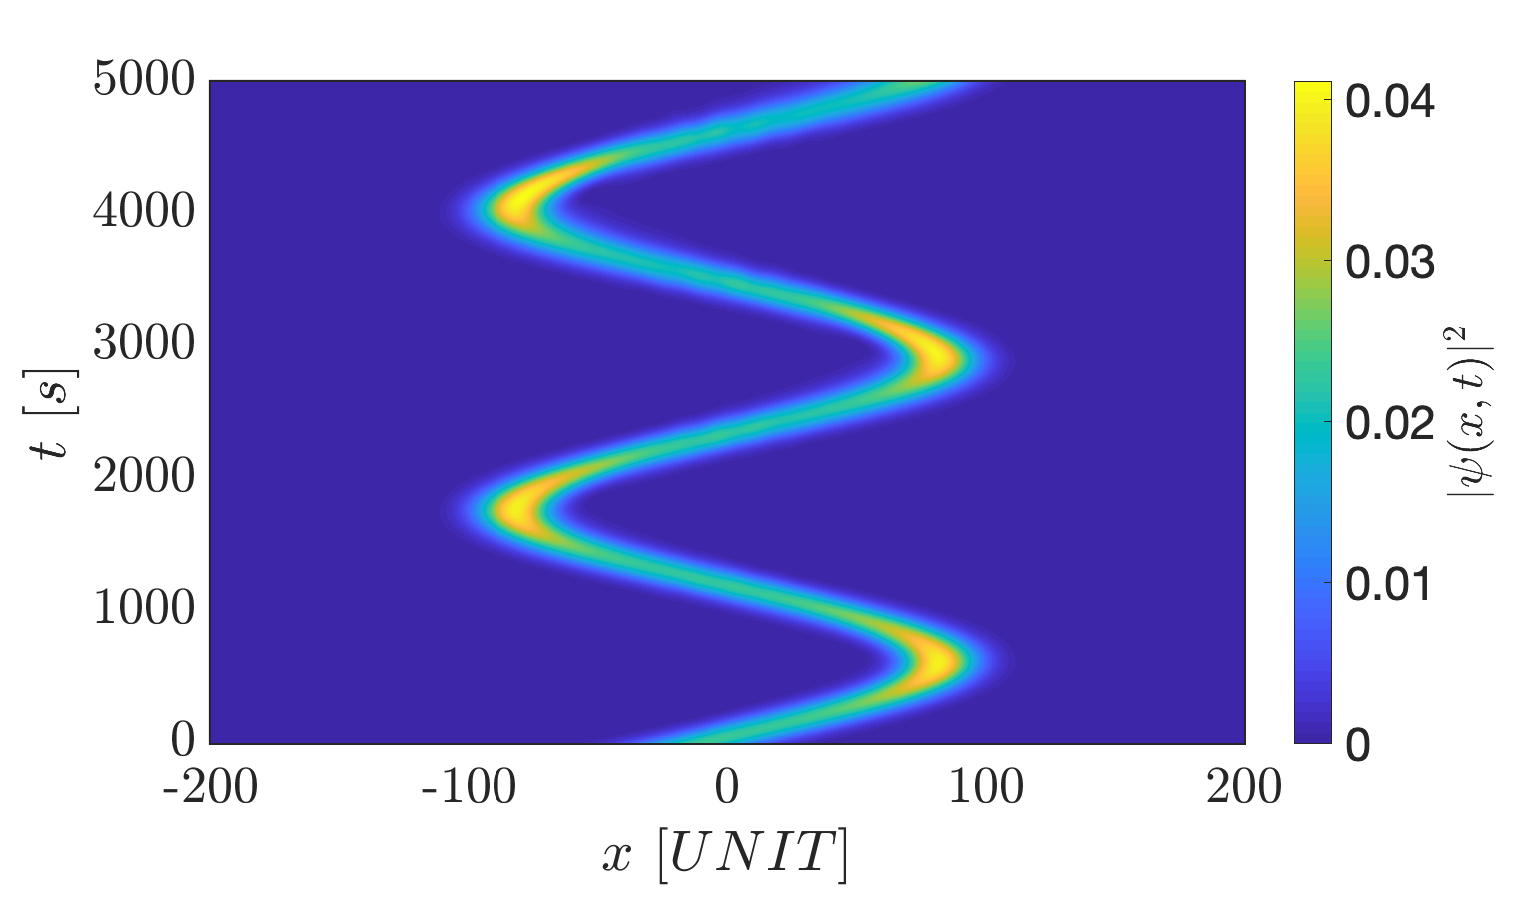
\includegraphics[width=\textwidth]{graphs/iii_evo_E>v0_psi.eps}
    \caption{$|\psi(\mbf{x}, t)|^2$ with respect to $\mbf{x}$ and t}
    \label{fig:iii_evo_E>v0_psi}
  \end{subfigure}
  ~
  \begin{subfigure}[t]{0.45\textwidth}
    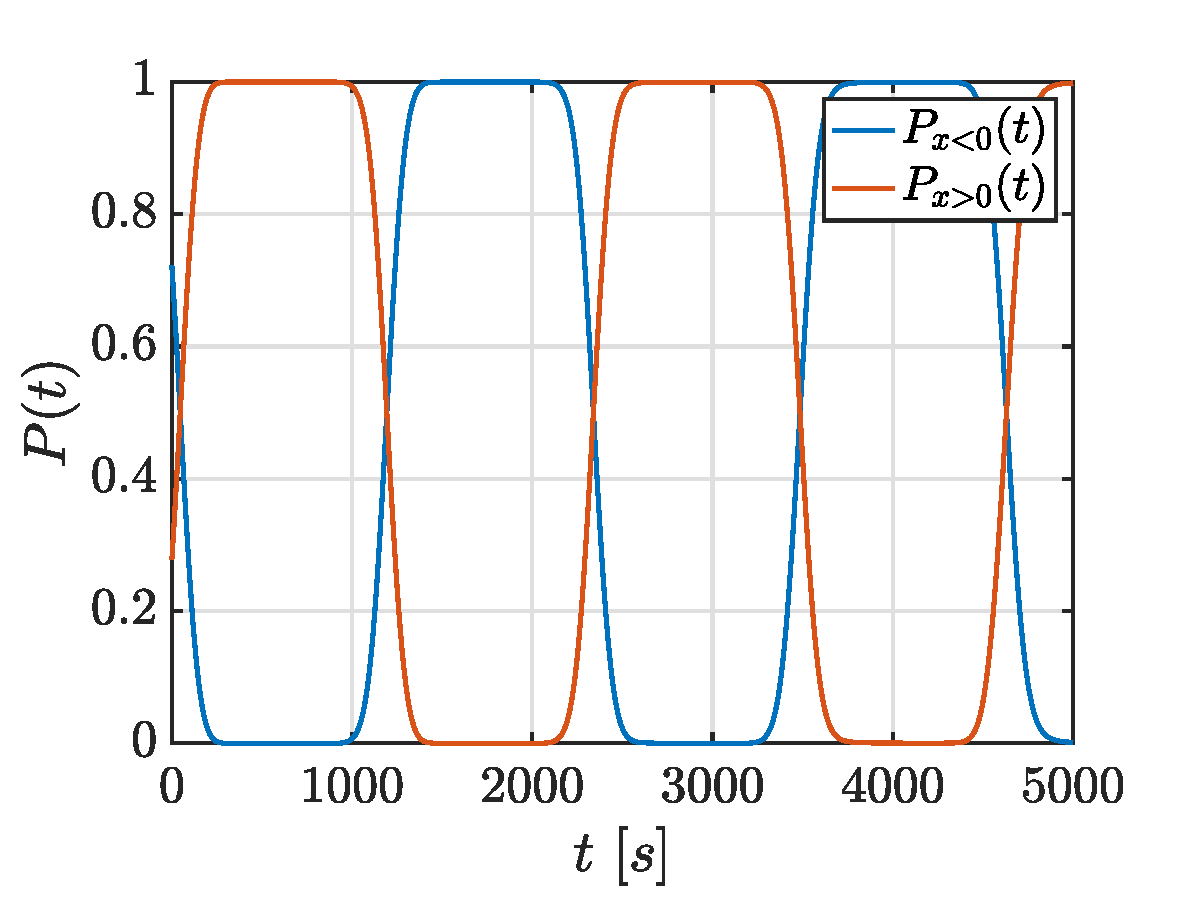
\includegraphics[width=\textwidth]{graphs/iii_evo_E>v0_prob.eps}
    \caption{$P(t)$ with respect to t}
    \label{fig:iii_evo_E>v0_prob}
  \end{subfigure}
  \caption{Evolution of the particle for $\Delta = 10$, which gives $E > V_0$}
  \label{fig:iii_evo_E>v0}
\end{figure}


\begin{figure}[h]
  \centering
  \begin{subfigure}[t]{0.45\textwidth}
    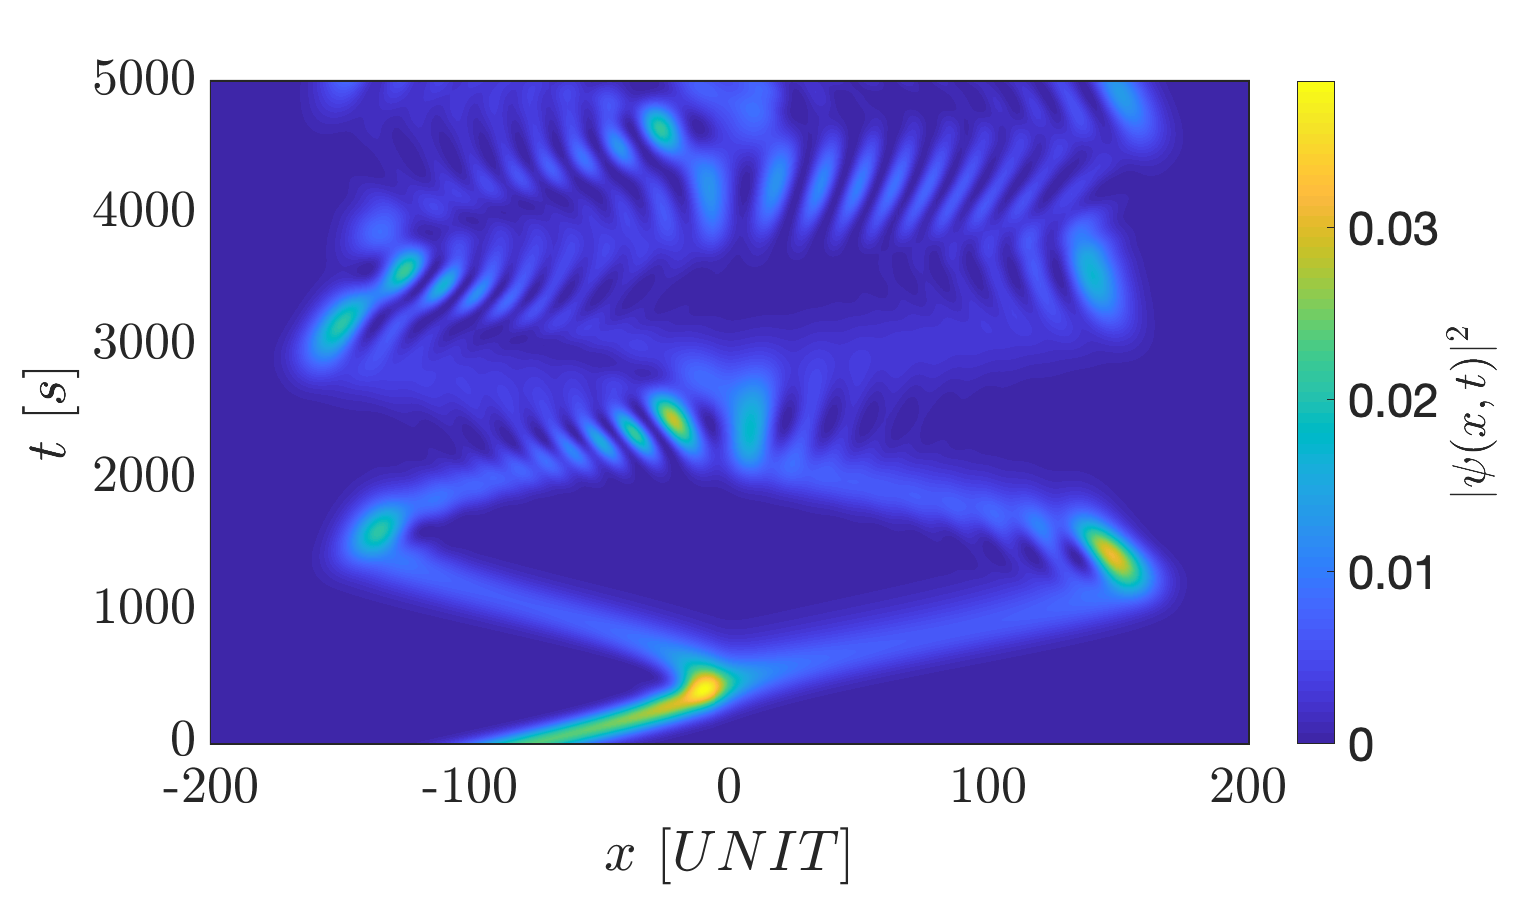
\includegraphics[width=\textwidth]{graphs/iii_evo_E=v0_psi.eps}
    \caption{$|\psi(\mbf{x}, t)|^2$ with respect to $\mbf{x}$ and t}
    \label{fig:iii_evo_E=v0_psi}
  \end{subfigure}
  ~
  \begin{subfigure}[t]{0.45\textwidth}
    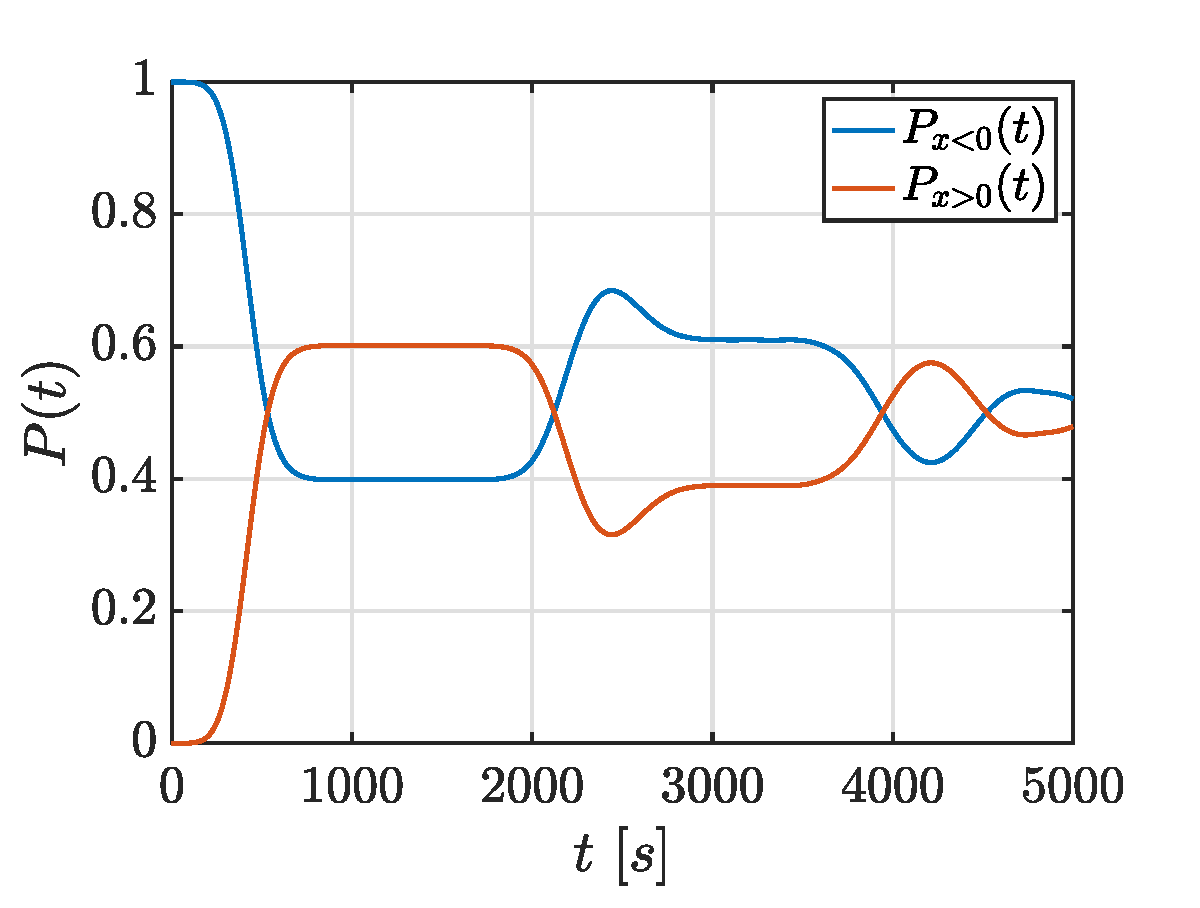
\includegraphics[width=\textwidth]{graphs/iii_evo_E=v0_prob.eps}
    \caption{$P(t)$ with respect to t}
    \label{fig:iii_evo_E=v0_prob}
  \end{subfigure}
  \caption{Evolution of the particle for $\Delta \approx 75.57$, which gives $E \approx V_0$}
  \label{fig:iii_evo_E=v0}
\end{figure}



\begin{figure}[h]
  \centering
  \begin{subfigure}[t]{0.45\textwidth}
    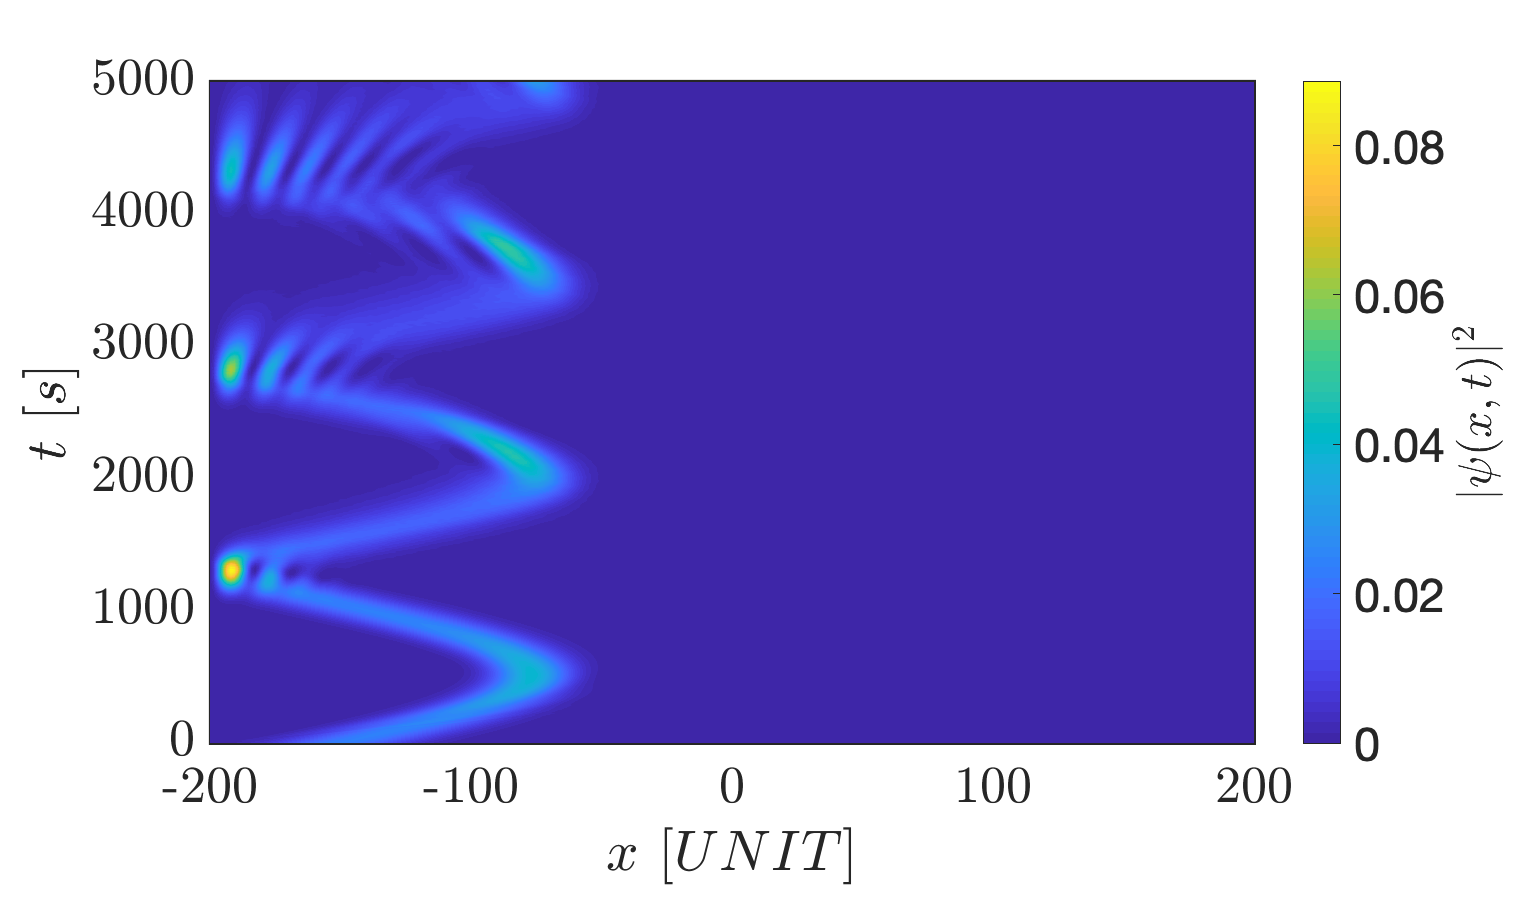
\includegraphics[width=\textwidth]{graphs/iii_evo_E<v0_psi.eps}
    \caption{$|\psi(\mbf{x}, t)|^2$ with respect to $\mbf{x}$ and t}
    \label{fig:iii_evo_E<v0_psi}
  \end{subfigure}
  ~
  \begin{subfigure}[t]{0.45\textwidth}
    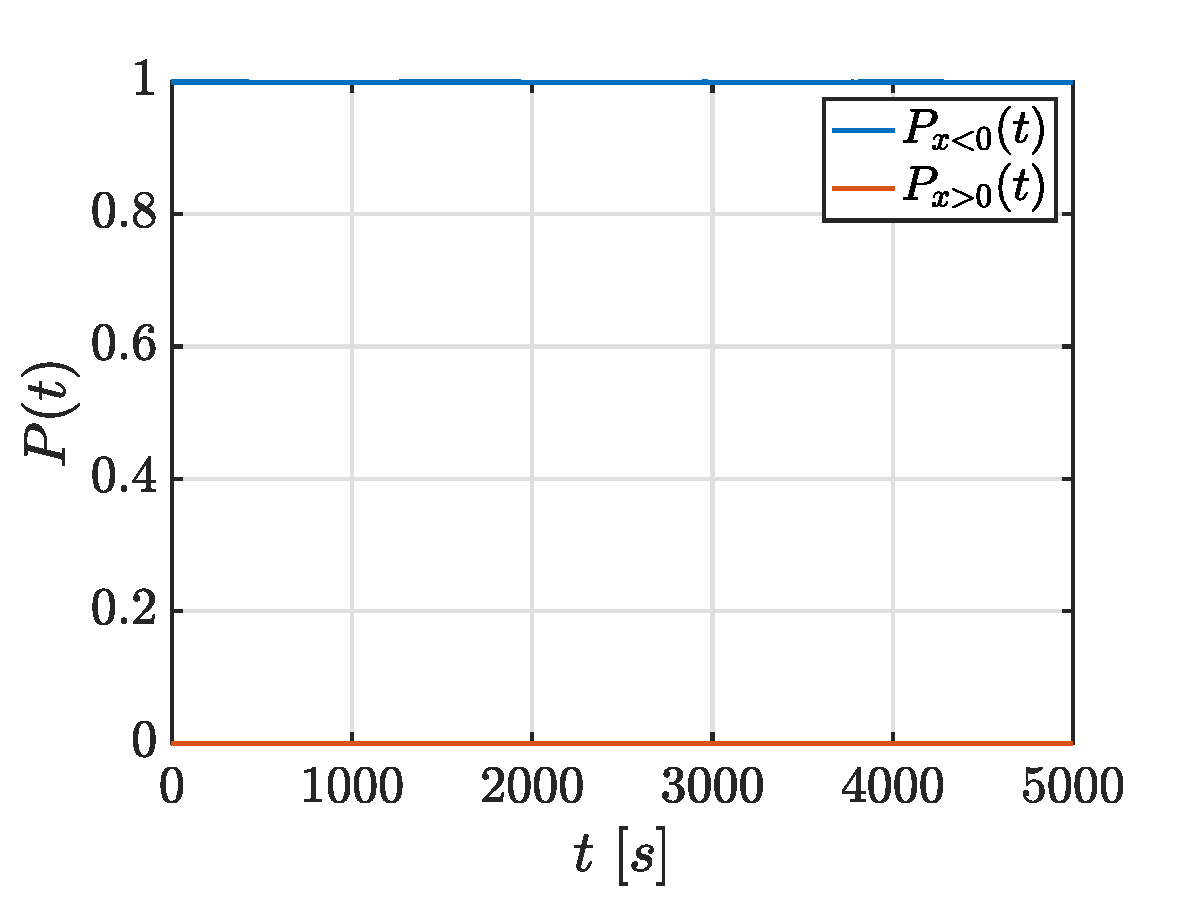
\includegraphics[width=\textwidth]{graphs/iii_evo_E<v0_prob.eps}
    \caption{$P(t)$ with respect to t}
    \label{fig:iii_evo_E<v0_prob}
  \end{subfigure}
  \caption{Evolution of the particle for $\Delta = 150$, which gives $E < V_0$}
  \label{fig:iii_evo_E<v0}
\end{figure}


\begin{figure}[h]
  \centering
  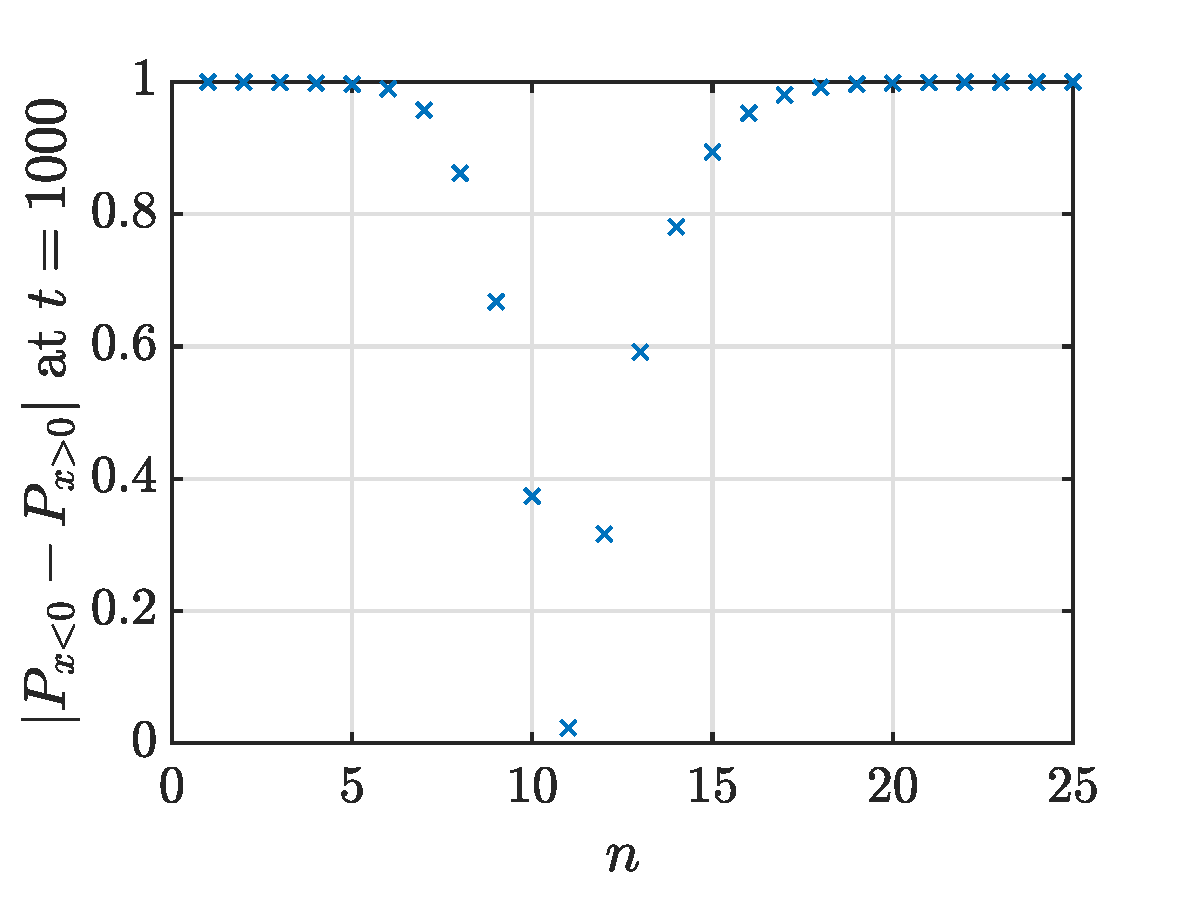
\includegraphics[width=0.5\textwidth]{graphs/iii_findn_n.eps}
  \caption{Difference of probabilities with respect to n}
  \label{fig:iii_findn_n}
\end{figure}


\begin{figure}[h]
  \centering
  \begin{subfigure}[t]{0.45\textwidth}
    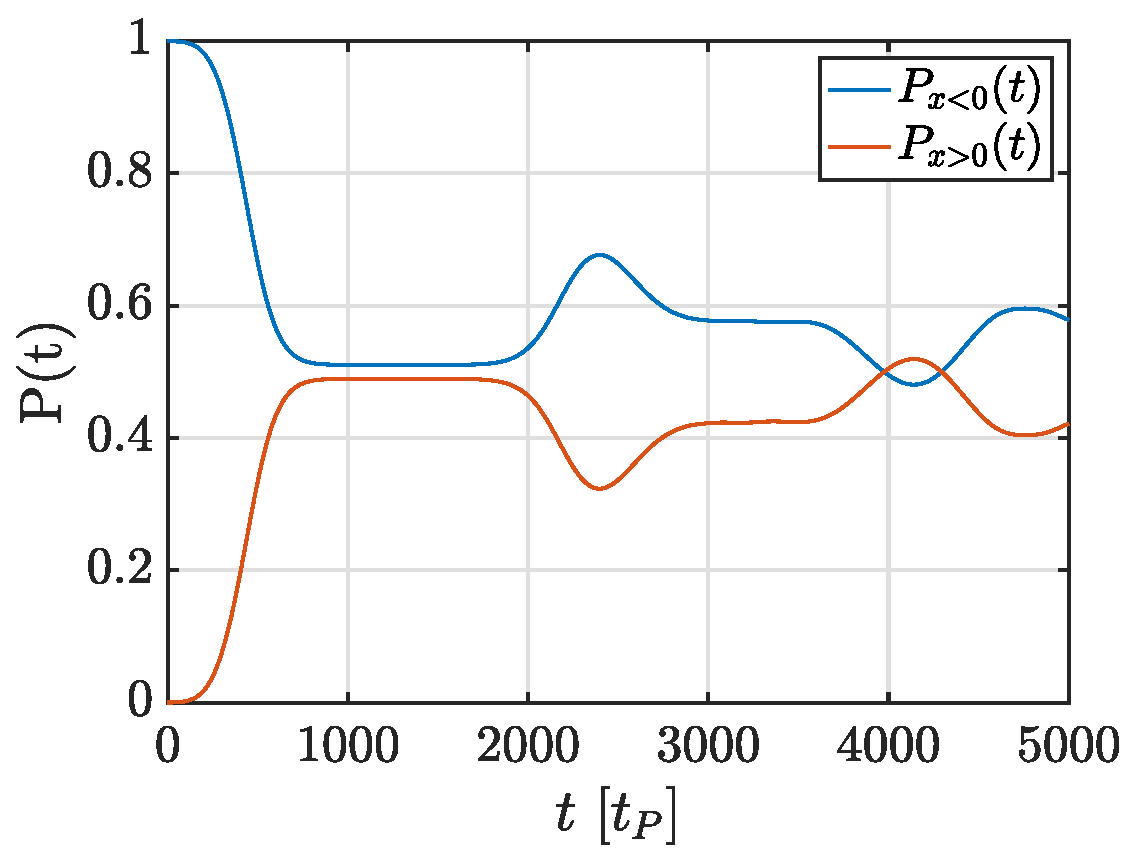
\includegraphics[width=\textwidth]{graphs/iii_findn_prob.eps}
    \caption{$|\psi(\mbf{x}, t)|^2$ with respect to $\mbf{x}$ and t}
    \label{fig:iii_findn_prob}
  \end{subfigure}
  ~
  \begin{subfigure}[t]{0.45\textwidth}
    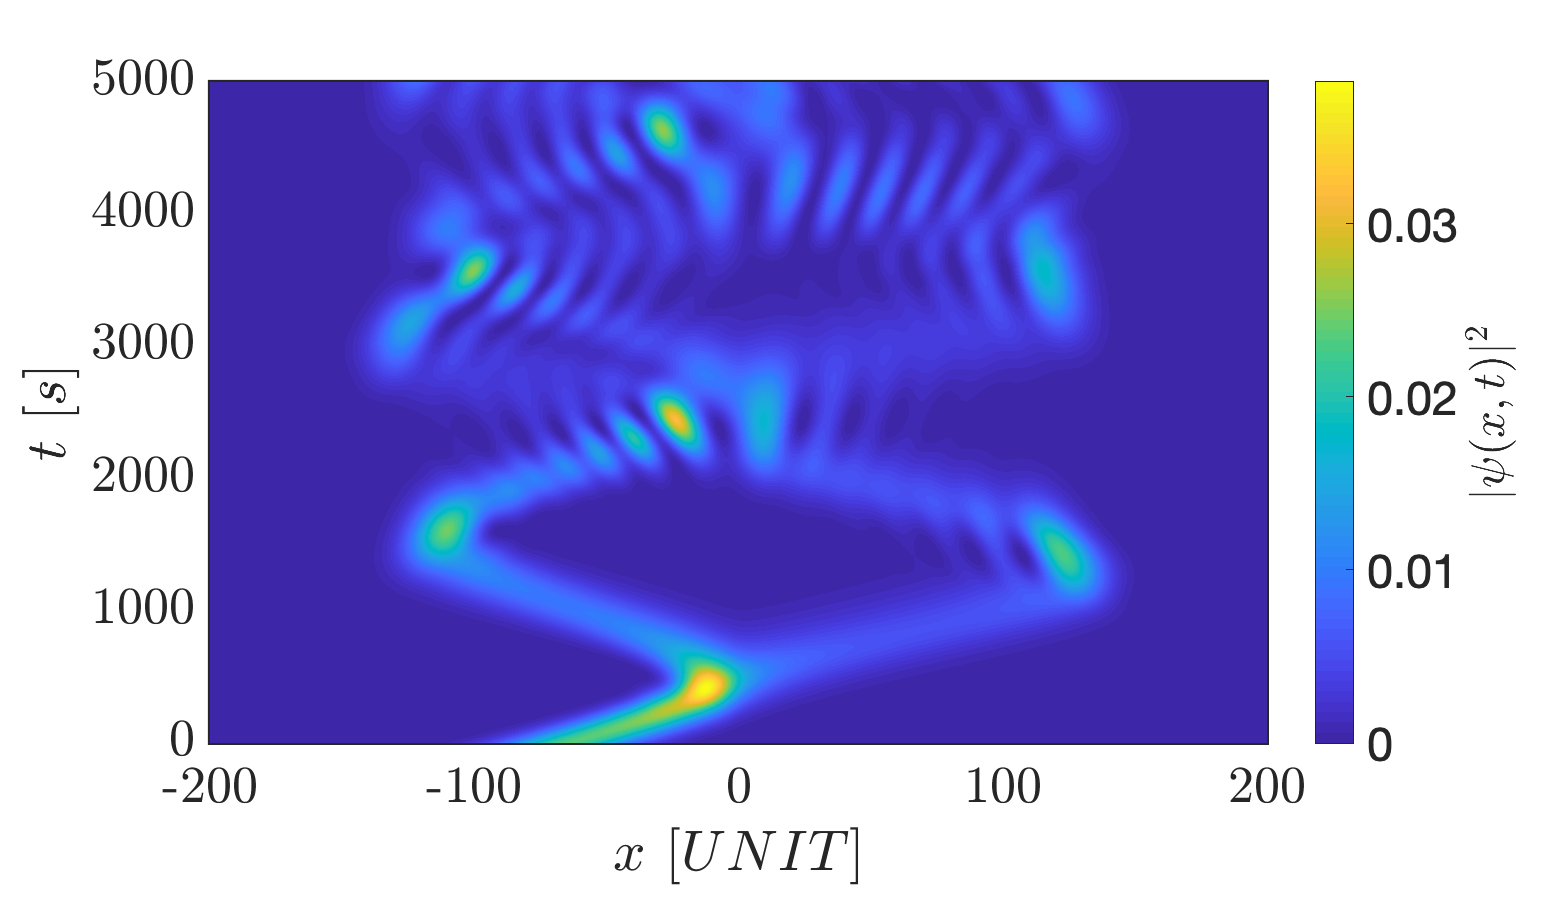
\includegraphics[width=\textwidth]{graphs/iii_findn_psi.eps}
    \caption{$P(t)$ with respect to t}
    \label{fig:iii_findn_psi}
  \end{subfigure}
  \caption{Evolution of the particle for $\Delta = 64$ with $n=11$}
  \label{fig:iii_findn}
\end{figure}



\section{Detection of a particle}





  % \newpage
  % \begin{thebibliography}{99}
  % \end{thebibliography}

\end{document}
